%\newcommand{\Exp}{\mathbb{E}}
\newcommand{\Cov}{\operatorname{Cov}}
\newcommand{\Var}{\operatorname{Var}}
\newcommand{\tr}{\operatorname{tr}}
\newcommand{\KL}{\operatorname{KL}}

% for commenting
\newcommand\TC[1]{\textcolor{blue}{[Trenton: #1]}}

% reset section counter
\setcounter{section}{0}

%\metadata{lecture ID}{Your names}{date}
\metadata{2}{Alexander Ke and Trenton Chang}{Jan 13th, 2021}

\sec{Review and overview}

In this lecture, we finish the proof on the asymptotic behavior of the excess risk, showing that it is asymptotically bounded in probability by $1/n$ (Section \ref{lec2:sec:asymp}). We then extend these results to the maximum likelihood estimation case and discuss the limitations of asymptotics. Motivated by these limitations, we introduce non-asymptotic analysis and apply it to uniform convergence.

Over the next few weeks, we will focus on how to bound the excess risk $L(\hat \theta) - L(\theta^*)$. On this we start with the asymptotic case and pick up from Lecture 1 by proving Parts 3 and 4 from Theorem~\ref{lec2:thm:last_time}.

\sec{Asymptotic analysis of the excess risk}
\label{lec2:sec:asymp}
In Lecture 1, we were introduced to Theorem \ref{lec2:thm:last_time} (this version has an additional Part 5, which is a consequence of Part 4).

\begin{theorem}
\label{lec2:thm:last_time}
Suppose that (a) $\hat{\theta}  \overset{p}{\to} \theta^{*}$ as $n \to \infty$ (i.e consistency of $\hat{\theta}$), (b) $\nabla^{2}L(\theta^{*})$ is full rank, and  (c) other appropriate regularity conditions hold. Then,
\begin{enumerate}
    \item $\sqrt{n} (\hat{\theta} - \theta^{*}) = O_P(1)$, i.e. for every $\epsilon > 0$, there is an $M$ such that $\sup_n \bbP (\| \sqrt{n} (\hat{\theta} - \theta^{*}) \|_2 > M) < \epsilon$. (This means that the sequence $\{ \sqrt{n} (\hat{\theta} - \theta^{*}) \}$ is ``bounded in probability".)
    
    \item  $\sqrt{n}(\hat{\theta}-\theta^{*}) \overset{d}{\to} \mathcal{N} \left(0, (\nabla^{2}L(\theta^{*}))^{-1}Cov(\ell((x,y), \theta^*)) (\nabla^{2}L(\theta^{*}))^{-1} \right)$.
     \item $n (L(\hat{\theta}) - L(\theta^{*})) = O_P(1)$.
    \item $n (L(\hat{\theta}) - L(\theta^{*})) \overset{d}{\to} \frac{1}{2} ||S||_{2}^{2}$ where $S \sim \mathcal{N} \left(0, (\nabla^{2}L(\theta^{*}))^{-1/2}Cov(\ell((x,y), \theta^*)) (\nabla^{2}L(\theta^{*}))^{-1/2} \right)$.
    \item $\lim_{n \to \infty} \E \left[ n (L(\hat \theta) - L(\theta^*)) \right] = \frac12 \tr\left( \nabla^2 L(\theta^*)^{-1} \Cov(\nabla \ell ((x, y), \theta^*) \right)$.
\end{enumerate}
\end{theorem}

\begin{proof}
Recall that Parts 1 and 2 were proven in Lecture 1, so we proceed with the proof of the remaining parts. Using a Taylor expansion of $L$ with respect to $\theta$ at $\theta^*$, we find
\begin{equation}
L(\hat \theta) = L(\theta^*) 
+ \langle \nabla L(\theta^*), \hat \theta - \theta^* \rangle 
+ \frac12 \langle \hat \theta - \theta^*, \nabla^2 L(\theta^*) (\hat \theta - \theta^*) \rangle + o(\|\hat \theta - \theta^*\|_2^2).
\end{equation}
Since $\theta^*$ is the minimizer of the population risk $L$, we know that $\nabla L(\theta^*) = 0$ and the linear term is equal to 0. Rearranging and multiplying by $n$, we can write
\begin{align}
n (L(\hat \theta) - L(\theta^*)) &= \frac{n}{2} \langle \hat \theta - \theta^*, \nabla^2 L(\theta^*) (\hat \theta - \theta^*) \rangle + o(\|\hat \theta - \theta^*\|_2^2) \\
&\approx \frac12 \langle \sqrt n(\hat \theta - \theta^*), \nabla^2 L(\theta^*) \sqrt n (\hat \theta - \theta^*) \rangle \\
&= \frac12 \left\|\nabla^2 L(\theta^*)^{1/2} \sqrt n(\hat \theta - \theta^*) \right\|_2^2,
\end{align}

where the last equality follows by the fact that for any vector $v$ and square matrix $A$ of appropriate dimensions, the inner product $\langle v, Av\rangle = v^T Av = \lVert A^{1/2}v \rVert_2^2$. Let $S = \nabla^2 L(\theta^*)^{1/2} \sqrt n(\hat \theta - \theta^*)$, i.e. the random vector inside the norm. By Part 2, we know the asymptotic distribution of $\sqrt n(\hat \theta - \theta^*)$ is Gaussian. Thus as $n \to \infty$, $n (L(\hat \theta) - L(\theta^*)) \overset d \to \frac12 \|S\|_2^2$ where
\begin{align}
    S &\sim \nabla^2 L(\theta^*)^{1/2} \cdot \cN \left(0, \nabla^2 L(\theta^*)^{-1} \Cov(\nabla \ell ((x, y), \theta^*) \nabla^2 L(\theta^*)^{-1} \right) \\
    &\stackrel{d}{=} \cN \left(0, \nabla^2 L(\theta^*)^{-1/2} \Cov(\nabla \ell ((x, y), \theta^*) \nabla^2 L(\theta^*)^{-1/2} \right).
\end{align}

This proves Part 4, and Part 3 follows directly from the definition of the $O_P$ notation. For Part 5, using the fact that the trace operator is invariant under cyclic permutations, the fact that $\E [S] = 0$, and some regularity conditions,
\begin{align}
    \lim_{n \to \infty} \E \left[ n (L(\hat \theta) - L(\theta^*)) \right] &= \frac12 \E\left[ \|S\|_2^2 \right] \\
    &= \frac12 \E \left[ \tr(S^\top S) \right] \\
    &= \frac12 \E \left[ \tr(S S^\top) \right] \\
    &= \frac12 \tr \left(\E[S S^\top] \right) \\
    &= \frac12 \tr \left( \Cov(S) \right) \\
    &= \frac12 \tr\left( \nabla^2 L(\theta^*)^{-1} \Cov(\nabla \ell ((x, y), \theta^*) \right).
\end{align}
\end{proof}

Theorem \ref{lec2:thm:last_time} is a powerful conclusion because once we know that $\sqrt{n}(\hat \theta  - \theta^*)$ is (asymptotically) Gaussian, we can easily work out the distribution of the excess risk. If we believe in our assumptions and $n$ is large enough such that we can assume $n \to \infty$, this allows us to analytically determine quantities of interest in almost any scenario (for example, if our test distribution changes). The key takeaway is that our parameter error $\hat{\theta} - \theta^*$ decreases in order $1/\sqrt{n}$ and the excess risk decreases in order $1/n$.

\subsec{Well-specified case}

Theorem \ref{lec2:thm:last_time} is powerful because it is general, avoiding any assumptions of a probabilistic model of our data. However in many applications, we assume a model of our data and we define the log-likelihood with respect to this model. Formally, suppose that we have a family of probability distributions $P_\theta$, parameterized by $\theta \in \Theta$, such that $P_{\theta_*}$ is the true data-generating distribution. This is known as the well-specified case. To make the results of Theorem \ref{lec2:thm:last_time} more applicable, we derive analogous results for this well-specified case in Theorem \ref{lec2:thm:applied}.

\begin{theorem}
\label{lec2:thm:applied}
    In addition to the assumptions of Theorem~\ref{lec2:thm:last_time}, suppose there exists a parametric model $P(y \mid x; \theta)$, $\theta \in \Theta$, such that $\{ y\sp{i} \mid x\sp{i} \}_{i=1}^n \sim P( y\sp{i} \mid x\sp{i} ; \theta_*)$ for some $\theta_* \in \Theta$. Assume that we performing maximum likelihood estimation (MLE), i.e. our loss function is the negative log-likelihood $\ell((x\sp{i}, y\sp{i}), \theta) = - \log P( y\sp{i} \mid x\sp{i} ; \theta)$. As before, let $\hat\theta$ and $\theta^*$ denote the minimizers of empirical risk and population risk respectively. Then
    \al{
    \label{lec2:eqn:applied1}
        \theta^* = \theta_*,
    }
    \al{
    \label{lec2:eqn:applied2}
        \E \left[ \nabla \ell ((x, y), \theta^*) \right] = 0,
    }
    \al{
    \label{lec2:eqn:applied3}
        \Cov \left( \nabla \ell ((x, y), \theta^*) \right) = \nabla^2 L(\theta^*), \text{ and}
    }
    \al{
    \label{lec2:eqn:applied4}
        \sqrt n (\hat \theta - \theta^*) \overset d \to \cN (0, \nabla^2 L(\theta^*)^{-1}).
    }
\end{theorem}

\textbf{Remark 1:} You may also have seen \eqref{lec2:eqn:applied4} in the following form: under the maximum likelihood estimation (MLE) paradigm, the MLE is asymptotically efficient in the Cramer-Rao lower bound. That is, the parameter error of the MLE estimate converges in distribution to $\mathcal{N}(0, \mathcal{I}(\theta)^{-1})$, where $\mathcal{I}(\theta)$ is the Fisher information matrix (in this case, equivalent to the risk Hessian $\nabla^2 L(\theta^*)$)~\cite{rice2006mathematical}.

\textbf{Remark 2:} \eqref{lec2:eqn:applied3} is also known as Bartlett's identity~\cite{percynotes}.

Although the proofs were not presented in live lecture, we include them here.

\begin{proof}
From the definition of the population loss,
\begin{align}
    L(\theta) &= \E \left[ \ell((x\sp{i}, y\sp{i}), \theta) \right]\\
    &= \E \left[ - \log P(y \mid x; \theta) \right] \\
    &= \E \left[ - \log P(y \mid x; \theta) + \log P(y \mid x; \theta_*) \right] + \E \left[ - \log P(y \mid x; \theta_*) \right] \\
    &= \E \left[ \log \frac{P(y \mid x; \theta_*)}{P(y \mid x; \theta)} \right] + \E \left[ - \log P(y \mid x; \theta_*) \right].
\end{align}
Notice that the second term is a constant which we will express as $\cH(y \mid x; \theta_*)$. We expand the first term using the tower rule (or law of total expectation):
\begin{align}
    L(\theta) &= \E \left[ \E \left[ \log \frac{P(y \mid x; \theta_*)}{P(y \mid x; \theta)} \biggr\vert x \right] \right] + \cH(y \mid x; \theta_*).
\end{align}
The term in the expectation is just the KL divergence between the two probabilities, so 
\begin{align}
    L(\theta) &= \E \left[ \KL \left( y \mid x; \theta_* \| y \mid x; \theta \right) \right] + \cH(y \mid x; \theta_*) \\
    &\geq \cH(y \mid x; \theta_*),
\end{align}
since KL divergence is always non-negative. Since $\theta_*$ makes the KL divergence term 0, it minimizes $L(\theta)$ and so $\theta_* \in \argmin_\theta L(\theta)$. However, the minimizer of $L(\theta)$ is unique because of consistency, so  we must have $\argmin_\theta L(\theta) = \theta^*$ which proves (\ref{lec2:eqn:applied1}).

For \eqref{lec2:eqn:applied2}, recall $\nabla L(\theta^*) = 0$, so we have
\begin{equation}
0 = \nabla L(\theta^*) = \nabla \E \left[ \ell((x\sp{i}, y\sp{i}), \theta^*) \right] = \E \left[ \nabla \ell((x\sp{i}, y\sp{i}), \theta^*) \right],
\end{equation}
where we can switch the gradient and expectation under some regularity conditions.

To prove \eqref{lec2:eqn:applied3}, we first expand the RHS using the definition of covariance and express the marginal distributions as integrals:
\begin{align}
    \Cov \left( \nabla \ell ((x, y), \theta^*) \right) &= \E \left[ \nabla \ell ((x, y), \theta^*) \nabla \ell ((x, y), \theta^*)^\top \right] \\
    &= \int P(x) \left( \int P(y \mid x; \theta^*) \nabla \log P( y\sp{i} \mid x\sp{i} ; \theta^*) \nabla \log P( y\sp{i} \mid x\sp{i} ; \theta^*)^\top dy \right) dx \\
    &= \int P(x) \left( \int \frac{\nabla P(y \mid x; \theta^*) \nabla P(y \mid x; \theta^*)^\top}{P(y \mid x; \theta^*)}dy \right) dx.
\end{align}
Now we expand the LHS using the definition of the population loss and differentiate repeatedly:
\begin{align}
    \nabla^2 L(\theta^*) &= \E \left[ \nabla^2 \log P(y \mid x; \theta^*) \right] \\
    &= \int P(x) \left( \int - \nabla^2 P(y \mid x; \theta^*) + \frac{\nabla P(y \mid x; \theta^*) \nabla P(y \mid x; \theta^*)^\top}{P(y \mid x; \theta^*)}dy  \right) dx.
\end{align}
Note that we can express 
\begin{equation} \int \nabla^2 P(y \mid x; \theta^*) dy = \nabla^2 \int P(y \mid x; \theta^*) dy = \nabla 1  = 0 \end{equation}
so we find
\begin{equation} \nabla^2 L(\theta^*) = \int P(x) \left( \int \frac{\nabla P(y \mid x; \theta^*) \nabla P(y \mid x; \theta^*)^\top}{P(y \mid x; \theta^*)}dy \right) dx = \Cov \left( \nabla \ell ((x, y), \theta^*) \right). \end{equation}

Finally, \eqref{lec2:eqn:applied4} follows directly from Part 2 of Theorem~\ref{lec2:thm:last_time} and \eqref{lec2:eqn:applied3}.
\end{proof}

Using similar logic to our proof of Part 4 and 5 of Theorem~\ref{lec2:thm:last_time}, we can see that $n (L(\hat \theta) - L(\theta^*)) \overset d \to \frac12 \|S\|_2^2$ where $S \sim N(0, I)$. Since a chi-squared distribution with $p$ degrees of freedom is defined as a sum of the squares of $p$ independent standard normals, it quickly follows that $2n (L(\hat \theta) - L(\theta^*)) \sim  \chi^2(p)$, where $\theta \in \R^p$ and $n \to \infty$. We can thus characterize the excess risk in this case using the properties of a chi-squared distribution:

\al{
    \lim_{n \to \infty} \E \left[ L(\hat \theta) - L(\theta^*) \right] = \frac{p}{2n}.
}

\sec{Introduction to non-asymptotic analysis}

This section introduces the concept of \textit{non-asymptotic analysis}. In the first half of this lecture and the previous lecture, we covered asymptotic analysis which tells you how learning algorithms behave as $n \to \infty$. This section will:
\begin{itemize}
    \item Motivate non-asymptotic analysis by highlighting a core limitation of asymptotic analysis.
    \item Introduce forms of Hoeffding's inequality, a concentration inequality used to derive bounds everywhere in non-asymptotic analysis.
\end{itemize}

\subsec{Motivation}
One limitation of asymptotic analysis is that our bounds often obscure dependencies on higher order terms. As an example, suppose we have a bound of the form
	\al{
		\frac{p}{2n} + o\left(\frac{1}{n}\right).
		\label{lec2:eqn:spicy_bound}
	}
(Here $o(\cdot)$ treats the parameter $p$ as a constant as $n$ goes to infinity.) 
We have no idea how large $n$ needs to be for asymptotic bounds to be ``reasonable." Compare two possible versions of \eqref{lec2:eqn:spicy_bound}: 
\begin{align}
    \frac{p}{2n} + \frac{1}{n^2} \quad \text{vs.} \quad \frac{p}{2n} + \frac{p^{100}}{n^2}.
\end{align}
Asymptotic analysis treats both of these bounds as the same, hiding the polynomial dependence on $p$ in the second bound. Clearly, the second bound is significantly more data-intensive than the first: we would need $n > p^{50}$ before $\frac{p^{100}}{n^2}$ is less than one. Since $p$ represents the dimensionality of the data, this may be an unreasonable assumption.

This is where non-asymptotic analysis can be helpful. Whereas asymptotic analysis uses large-sample theorems such as the central limit theorem and the law of large numbers to provide convergence guarantees, non-asymptotic analysis relies on concentration inequalities to develop alternative techniques for reasoning about the performance of learning algorithms.

\subsec{Clarifications on notation}

For the rest of this course, we will use ``big-O" notation in the following sense: every occurrence of $O(x)$ is a placeholder for some function $f(x)$ such that for every $x$, $|f(x)| \leq Cx$ for some absolute/universal constant $C$. (The difference with traditional ``big-O" notation is that we do not need to send $n \to \infty$ in order to define ``big-O".)

Also, for any $a, b \geq 0$, we will let $a \lesssim b$ mean that there is some absolute constant $c > 0$ such that $a \leq cb$.

In this lecture, we are not going to care about the constants much, so the absolute constants in the bounds may not be tight.

\subsec{Preliminaries: Hoeffding's inequality}\label{lec2:subsec:hoeffding}

We provide a brief overview of Hoeffding's inequality, a foundational concentration inequality:

\begin{theorem}[Hoeffding's inequality]
    Let $X_1, X_2, \dots, X_n$ be i.i.d. real-valued random variables drawn from some distribution, such that $a_i \leq X_i \leq b_i$ almost surely. Define $\bar{X} = \frac{1}{n}\sum_{i=1}^n X_i$, and let $\mu = \E [\bar{X}]$. Then for any $\varepsilon > 0$,
    \al {
    \Pr \left[ |\bar{X} - \mu | \leq \varepsilon \right] \geq 1 - 2  \exp\left(\frac{-2n^2\varepsilon^2}{\sum_{i=1}^n (b_i - a_i)^2}\right). \label{lec2:eqn:hoeffding}
    }
\end{theorem}

Note that the demoninator within the exponential term, $\sum_{i=1}^n (b_i - a_i)^2$, can be thought of as an upper bound or proxy for the variance $\Var(X_i)$. In fact, under the i.i.d. assumption, we can show
\begin{align}
    \Var\left(\bar{X} \right) &= \frac{1}{n^2}\sum_{i=1}^n \Var(x_i) \leq \frac{1}{n^2}\sum_{i=1}^n (b_i - a_i)^2.
\end{align}

Let $\sigma^2 = \frac{1}{n^2}\sum_{i=1}^n (b_i - a_i)^2$. If we take $\varepsilon = O(\sigma \sqrt{\log{n}}) = \sigma \sqrt{c \log n}$; i.e. $\varepsilon$ bounded above by some large (i.e., $c \geq 10$) multiple of the standard deviation of the $x_i$'s times $\sqrt{\log{n}}$, we can substitute this value of $\varepsilon$ into \eqref{lec2:eqn:hoeffding} to reach the following conclusion: 
\begin{align}
    \Pr \left[ |\bar{X} - \mu| \leq \varepsilon \right] &\geq 1 - 2\exp\left(\frac{-2 \varepsilon^2}{\sigma^2}\right)\\
    &= 1 - 2 \exp(-2 c \log n)\\
    &= 1 - 2 n^{-2c}
\end{align}

We can see that as $n$ grows, the right-most term tends to zero such that $\Pr[|\bar{X} - \mu| \leq \varepsilon]$ very quickly approaches 1. Intuitively, this result tells us that, with high probability, the sample mean $\bar{X}$ will not be ``much farther" from the population mean $\mu$ by some sublogarithmic ($\sqrt{c \log n}$) factor of the standard deviation.\footnote{This is with the caveat, of course, that $\sigma$ is not exactly standard deviation but a loose upper bound on standard deviation.} Thus, we can restate the above claim we reached as follows:

\begin{remark}
    For sufficiently large $n$, $|\bar{X} - \mu | \leq O(\sigma \sqrt{\log{n}})$ with high probability.
\end{remark}

\begin{remark}\label{lec2:rem:hoeffding}
    If, in addition, we have $a_i = -O(1)$ and $b_i = O(1)$, then $\sigma^2 = O \left( \frac{1}{n}\right)$, and $|\bar{X} - \mu | \leq O\left(\sqrt{\frac{\log n}{n}}\right) = \tilO\left(\frac{1}{\sqrt{n}}\right)$.\footnote{$\tilO$ is analogous to Big-$O$ notation, in that $\tilO$ hides logarithmic factors. That is; if $f(n) = O(\log n)$, then $f(n) = \tilO(1)$.}
\end{remark}

Remark~\ref{lec2:rem:hoeffding} provides a compact form of the Hoeffding bound that we can use when the $X_i$ are bounded almost surely. Now, we will apply this mathematical machinery to learning theory.

\sec{Introduction to uniform convergence}

One problem area where non-asymptotic analysis is useful is \emph{uniform convergence.} A central goal of learning theory is to bound the \emph{excess risk} $L(\hat{\theta}) - L(\theta^*)$. This is important as we don't want the expected risk of our ERM to be much larger than the expected risk of the best possible model. As we will see in the remainder of this section, uniform convergence is a technique that helps us achieve such bounds.

Uniform convergence is a property of a parameter set $\Theta$, which gives us bounds of the form
\al{
    \Pr \left[|\hat{L}(\theta) - L(\theta)| \geq \varepsilon \right] \leq \delta; \; \forall \theta \in \Theta.\label{lec2:eqn:uc}
}
In other words, uniform convergence tells us that for any choice of $\theta$, our empirical risk is always close to our population risk with high probability. Let's look at a motivating example for why this type of bound is useful.

\subsec{Motivation: Uniform convergence implies generalization}

Consider the standard supervised learning setup where we have some i.i.d. $(x\sp{i}, y\sp{i})$. Furthermore, assume that we have a bounded loss function; specifically, suppose that $0 \leq \ell((x, y); \theta) \leq 1$, as in the case of the zero-one loss function. We show that uniform convergence implies generalization.

First, via telescoping sums, we can decompose the excess risk into three terms:
\al{
    L(\hat{\theta}) - L(\theta^*) = \underbrace{L(\hat{\theta}) - \hat{L}(\hat{\theta})}_\text{\circled{1}} + \underbrace{\hat{L}(\hat{\theta}) - \hat{L}(\theta^*)}_\text{\circled{2}} + \underbrace{\hat{L}(\theta^*) - L(\theta^*)}_\text{\circled{3}}.
}
We know that $\hat{L}(\hat{\theta}) - \hat{L}(\theta^*) \leq 0$ since $\hat{\theta}$ is a minimizer of $\hat{L}$. This allows us to write
\begin{align}
L(\hat{\theta}) - L(\theta^*) &\leq |L(\hat{\theta}) - \hat{L}(\hat{\theta})| + \hat{L}(\hat{\theta}) - \hat{L}(\theta^*) + |\hat{L}(\theta^*) - L(\theta^*)|\\
&\leq |L(\hat{\theta}) - \hat{L}(\hat{\theta})| + 0 + |\hat{L}(\theta^*) - L(\theta^*)|\\
&\leq 2\;\sup_{\theta \in \Theta } |L(\theta) - \hat{L}(\theta)|. \label{lec2:eqn:1}
\end{align}
This result tells us that if $\sup_{\theta \in \Theta } |L(\theta) - \hat{L}(\theta)|$ is small (say, less than $\varepsilon/2$), then excess risk $L(\hat{\theta}) - L(\theta^*)$ is less than $\varepsilon$. But this is exactly in the form of the bound in \eqref{lec2:eqn:uc}. Hence, if we can show that a parameter family exhibits uniform convergence, we can get a bound on excess risk as well.

For future references, Equation~\eqref{lec2:eqn:1} can be strengthened straightforwardly into the following with slightly more careful treatment of the signs of each term:
\begin{align}
L(\hat{\theta}) - L(\theta^*) \le |\hat{L}(\theta^*) - L(\theta^*)|+  L(\hat{\theta}) - \hat{L}(\hat{\theta})  \le |\hat{L}(\theta^*) - L(\theta^*)|+ \sup_{\theta \in \Theta} \left(L(\hat{\theta}) - \hat{L}(\hat{\theta})\right)\label{lec2:eqn:2}
\end{align}
This will make some of our future derivations technically slightly more convenient, but the nuanced difference between Equations~\eqref{lec2:eqn:1} and~\eqref{lec2:eqn:2} does not change the fundamental idea and the discussions in this lecture. 

Let us try to apply our knowledge of concentration inequalities to this problem. Earlier we assumed that $\ell((x, y); \theta)$ is bounded, so we can bound $\circled{3}$ by $\tilO\left(\frac{1}{\sqrt{n}}\right)$ via Hoeffding's inequality (Remark \ref{lec2:rem:hoeffding}). However, we cannot apply the same concentration inequality to $\circled{1}$: since $\hat{\theta}$ is data-dependent by definition, the i.i.d. assumption no longer holds. (To see this, note that $\hat\theta$ depends on the training dataset $(x\sp{i}, y\sp{i})$, so the terms in $\hatL (\theta)$, $\ell ((x\sp{i}, y\sp{i}); \hat\theta)$, all depend on the training dataset too.) This is concerning: it is certainly possible that $L(\hat{\theta}) - \hat{L}(\hat{\theta})$ is large. You've probably encountered this yourself when a model exhibits low training loss, but high validation/testing loss. 

\subsec{Deriving uniform convergence bounds}

Uniform convergence is one way we can fix this issue. The high-level idea is as follows: 
\begin{itemize}
    \item Suppose we have a bound of the form $\Pr[|\hat{L}(\theta) - L(\theta)| \geq \varepsilon'] \leq \delta'$ for some single, fixed choice of $\theta$.
    \item If we know \emph{all possible values of $\theta$} in advance, we can use the above bound to create a more general bound over all values of $\theta$.
\end{itemize}
In particular, we can use the union-bound inequality to create the general bound described in the second bullet point, using the bound in the first bullet point:
\al{
    \Pr \left[\forall \theta \in \Theta; |\hat{L}(\theta) - L(\theta)| \geq \varepsilon' \right] \leq \sum_{\theta \in \Theta} \Pr \left[|\hat{L}(\theta) - L(\theta)| \geq \varepsilon' \right].
}
We can then use Hoeffding's inequality to deal with the summands as $\theta$ there is no longer data-dependent. We'll talk more in future lectures about proving statements of this form.

\subsec{Intuitive Interpretation of Uniform Convergence.}

Since uniform convergence implies generalization, if we know that population risk and empirical risk are always ``close," then excess risk is ``small" as well (Figure \ref{lec2:fig:uc}). In fact, it is possible to show that not only is $L(\theta)$ ``close" to $\hat{L}(\theta)$ for sufficiently large data, but that the ``shape" of $\hat{L}$ is ``close" to the shape of $L$ as well (Figure \ref{lec2:fig:shape}). This holds for the convex case; furthermore, there are conditions under which this holds in the non-convex case, for which a rigorous treatment can be found in~\cite{mei2017landscape}.\\\\
\emph{Figure design and some wording in this section was inspired by~\cite{percynotes, thomasliu2018}.}

\begin{figure}[t]
    \centering
    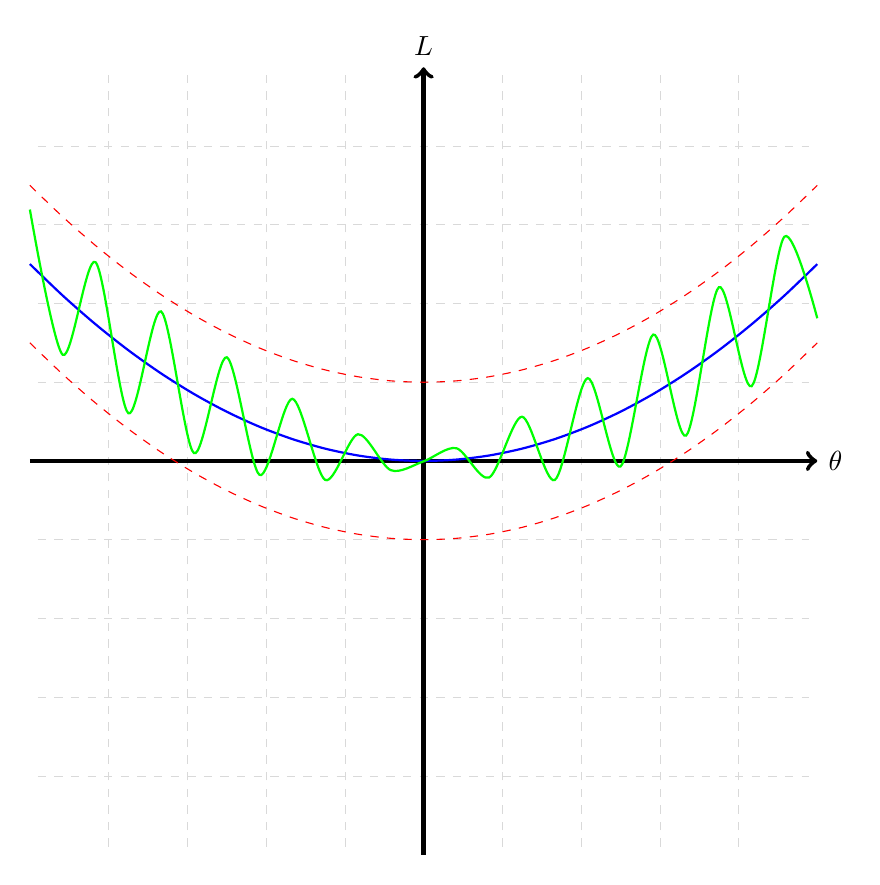
\begin{tikzpicture}
    \draw[help lines, color=gray!30, dashed] (-4.9,-4.9) grid (4.9,4.9);
    \draw[->,ultra thick] (-5,0)--(5,0) node[right]{$\theta$};
    \draw[->,ultra thick] (0,-5)--(0,5) node[above]{$L$};
    \draw[blue, thick]   plot[smooth,domain=-5:5] (\x, {0.1* (\x*\x)});
    \draw[red, dashed]   plot[smooth,domain=-5:5] (\x, {0.1* (\x*\x) + 1});
    \draw[red, dashed]   plot[smooth,domain=-5:5] (\x, {0.1* (\x*\x) - 1});
    \draw[green, thick]   plot[smooth,domain=-5:5] (\x, {0.1* (\x*\x) + 0.8 * sin(3000 * \x)});
\end{tikzpicture}
    \caption{Empirical risk landscape under uniform convergence: \textcolor{green}{Green:} empirical risk, \textcolor{blue}{blue:} population risk, \textcolor{red}{red, dashed:} $\varepsilon$ additive error bounds for excess risk.}
    \label{lec2:fig:uc}
\end{figure}

\begin{figure}[t]
    \centering
    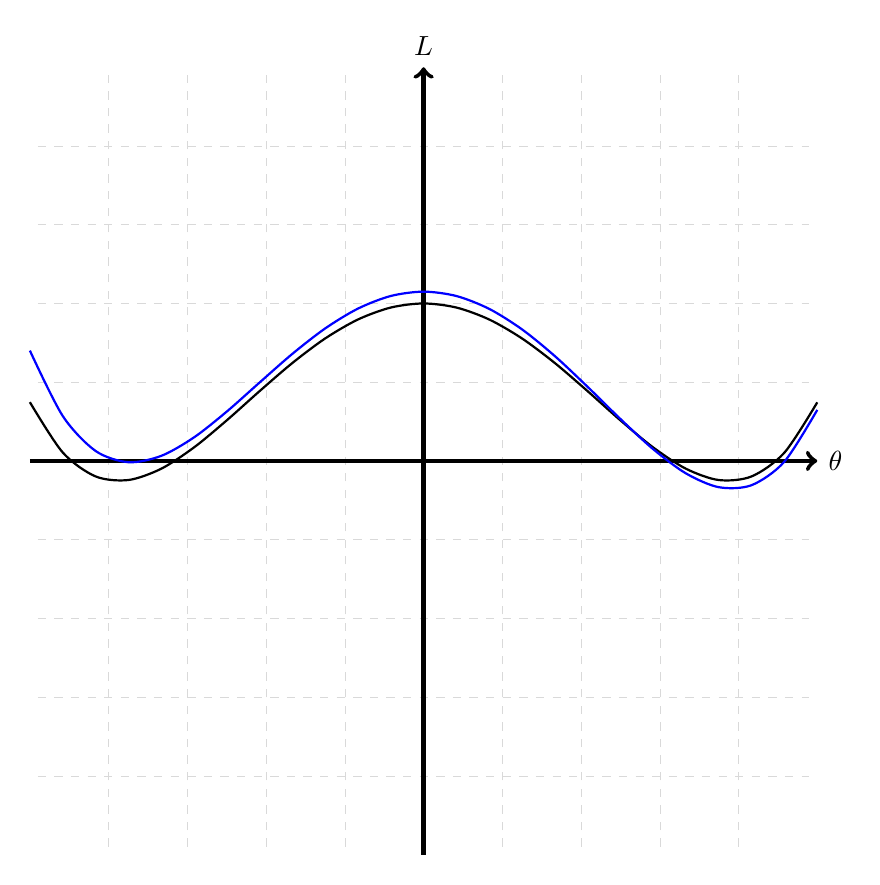
\begin{tikzpicture}
    \draw[help lines, color=gray!30, dashed] (-4.9,-4.9) grid (4.9,4.9);
    \draw[->,ultra thick] (-5,0)--(5,0) node[right]{$\theta$};
    \draw[->,ultra thick] (0,-5)--(0,5) node[above]{$L$};
    \draw[black, thick]   plot[smooth,domain=-5:5] (\x, {0.01*\x*\x*\x*\x - 0.3*\x*\x + 2});
    \draw[blue, thick]   plot[smooth,domain=-5:5] (\x, {0.011*\x*\x*\x*\x -0.003*\x*\x*\x - 0.32*\x*\x + 2.15});
\end{tikzpicture}
    \caption{Empirical risk landscape under uniform convergence: \textcolor{blue}{Blue:} empirical risk, \textcolor{black}{black:} population risk.}
    \label{lec2:fig:shape}
\end{figure}
